\documentclass{standalone}
\usepackage{tikz}
\usetikzlibrary{patterns, positioning}
\usepackage[sfdefault]{ClearSans} %% option 'sfdefault' activates Clear Sans as the default text font
\usepackage[T1]{fontenc}

\begin{document}
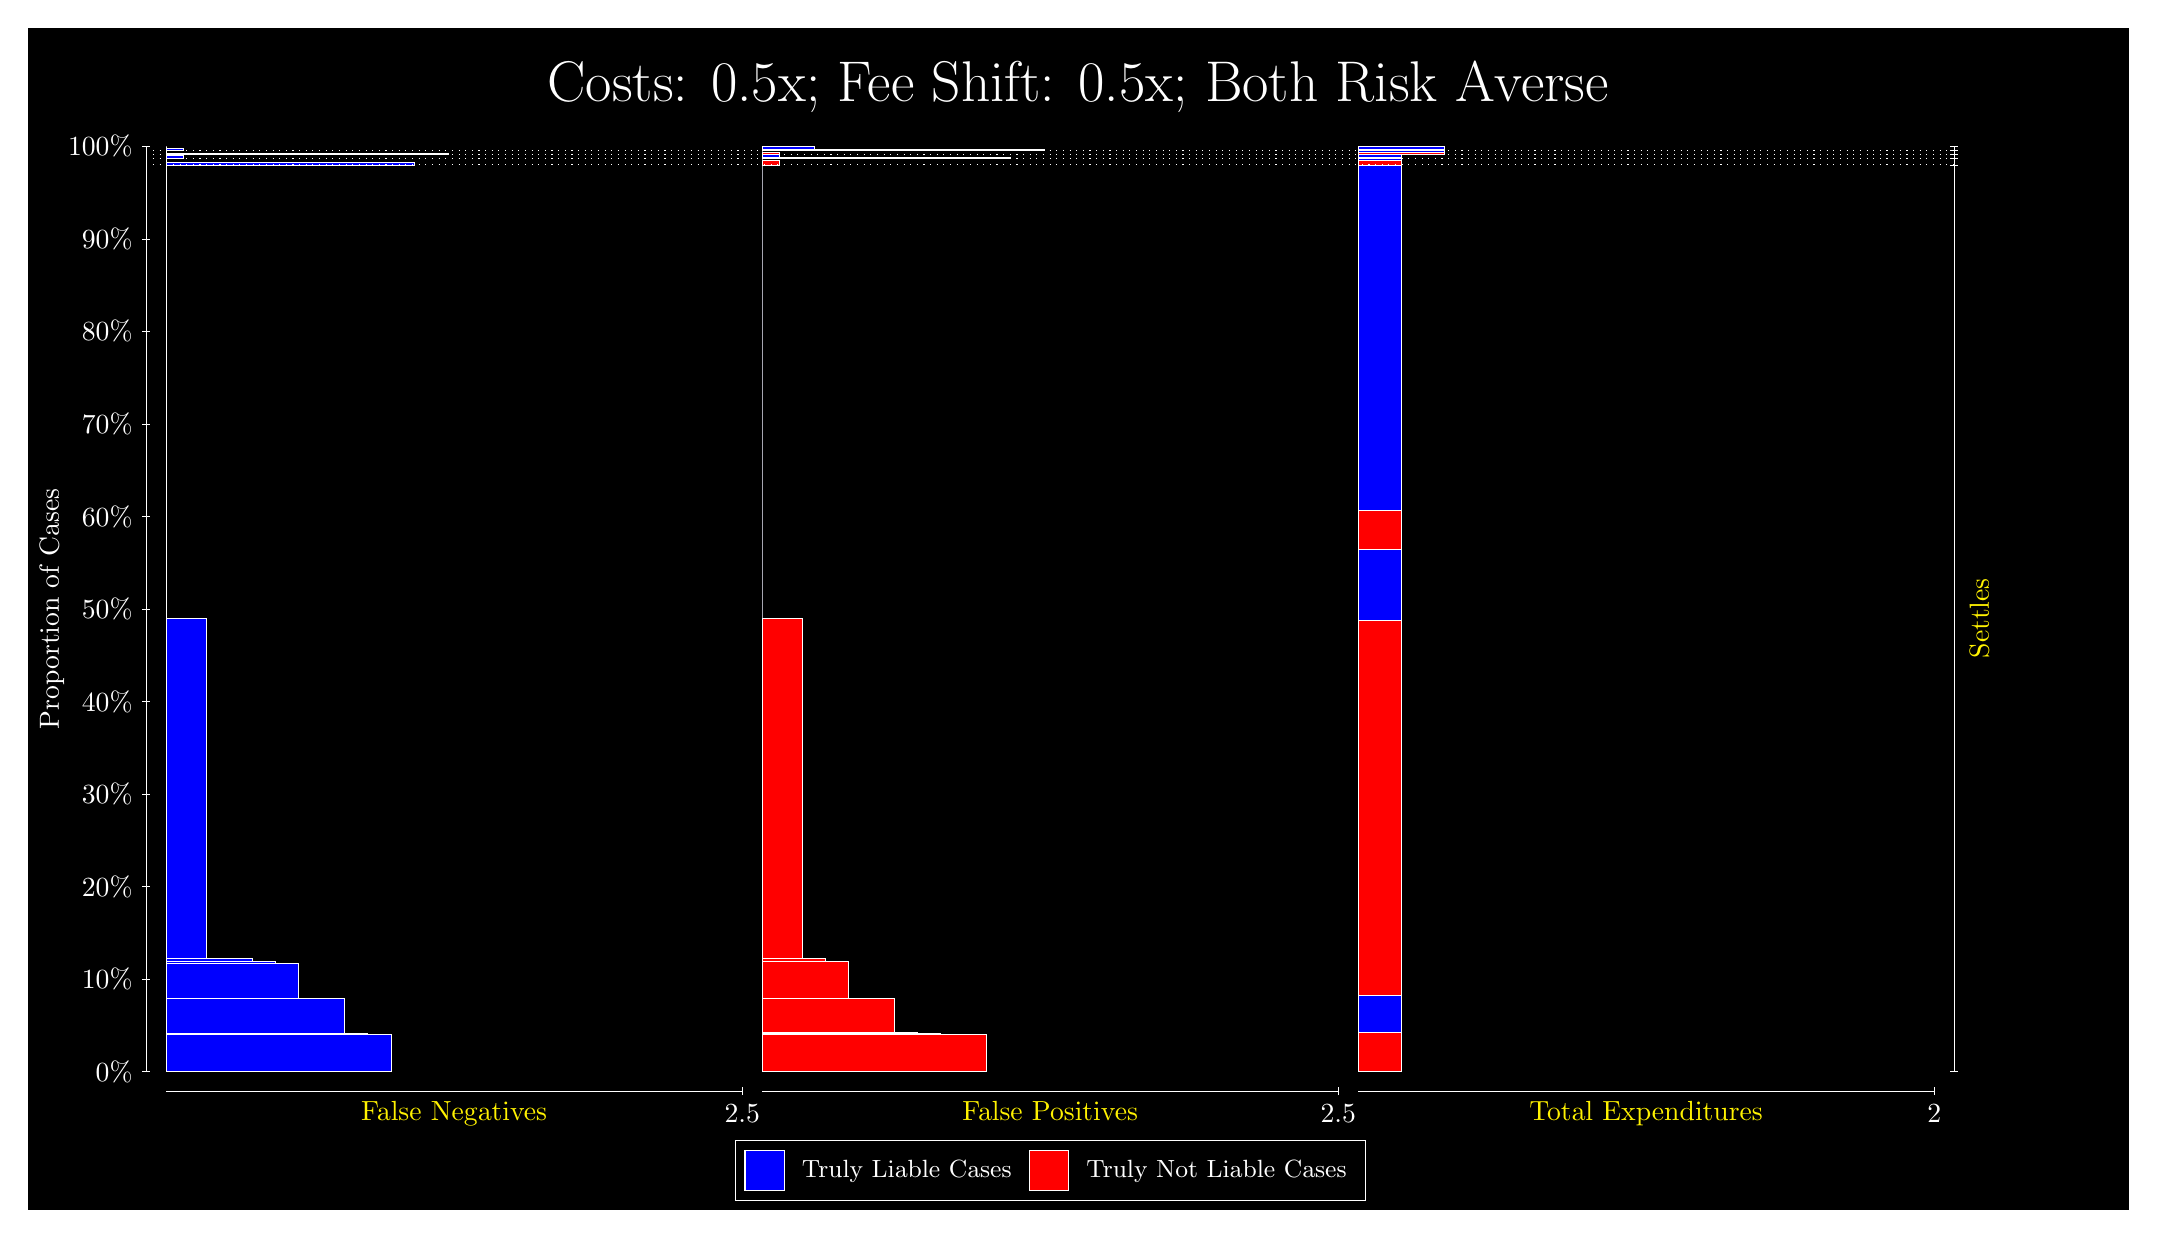
\begin{tikzpicture}
\draw[fill=black] (0,0) rectangle (26.667,15);
\draw[text=white] (0,13.5) rectangle (26.667,15) node[midway] {\huge Costs: 0.5x; Fee Shift: 0.5x; Both Risk Averse};
\draw[white, very thin] (1.5,1.75) -- (1.5,13.5);
\node[rotate=90, text=white, anchor=center] at (0.3, 7.625) {Proportion of Cases};
\draw[white, very thin] (1.45,1.75) -- (1.55,1.75);
\node[text=white, anchor=east] at (1.45, 1.75) {0\%};
\draw[white, very thin] (1.45,2.925) -- (1.55,2.925);
\node[text=white, anchor=east] at (1.45, 2.925) {10\%};
\draw[white, very thin] (1.45,4.1) -- (1.55,4.1);
\node[text=white, anchor=east] at (1.45, 4.1) {20\%};
\draw[white, very thin] (1.45,5.275) -- (1.55,5.275);
\node[text=white, anchor=east] at (1.45, 5.275) {30\%};
\draw[white, very thin] (1.45,6.45) -- (1.55,6.45);
\node[text=white, anchor=east] at (1.45, 6.45) {40\%};
\draw[white, very thin] (1.45,7.625) -- (1.55,7.625);
\node[text=white, anchor=east] at (1.45, 7.625) {50\%};
\draw[white, very thin] (1.45,8.8) -- (1.55,8.8);
\node[text=white, anchor=east] at (1.45, 8.8) {60\%};
\draw[white, very thin] (1.45,9.975) -- (1.55,9.975);
\node[text=white, anchor=east] at (1.45, 9.975) {70\%};
\draw[white, very thin] (1.45,11.15) -- (1.55,11.15);
\node[text=white, anchor=east] at (1.45, 11.15) {80\%};
\draw[white, very thin] (1.45,12.325) -- (1.55,12.325);
\node[text=white, anchor=east] at (1.45, 12.325) {90\%};
\draw[white, very thin] (1.45,13.5) -- (1.55,13.5);
\node[text=white, anchor=east] at (1.45, 13.5) {100\%};

\draw[white, very thin] (24.457,1.75) -- (24.457,13.5);
\draw[white, very thin] (24.407,1.75) -- (24.507,1.75);
\node[anchor=west] at (24.407, 1.75) {};
\draw[white, very thin] (24.407,13.265) -- (24.507,13.265);
\node[anchor=west] at (24.407, 13.265) {};
\draw[white, very thin] (24.407,13.347) -- (24.507,13.347);
\node[anchor=west] at (24.407, 13.347) {};
\draw[white, very thin] (24.407,13.4) -- (24.507,13.4);
\node[anchor=west] at (24.407, 13.4) {};
\draw[white, very thin] (24.407,13.444) -- (24.507,13.444);
\node[anchor=west] at (24.407, 13.444) {};
\draw[white, very thin] (24.407,13.5) -- (24.507,13.5);
\node[anchor=west] at (24.407, 13.5) {};

\draw[white, very thin, fill=blue] (1.75,1.75) rectangle (4.6044,2.2189);
\draw[white, very thin, fill=blue] (1.75,2.2189) rectangle (4.3116,2.2336);
\draw[white, very thin, fill=blue] (1.75,2.2336) rectangle (4.0188,2.6843);
\draw[white, very thin, fill=blue] (1.75,2.6843) rectangle (3.4333,3.1209);
\draw[white, very thin, fill=blue] (1.75,3.1209) rectangle (3.1406,3.1518);
\draw[white, very thin, fill=blue] (1.75,3.1518) rectangle (2.8478,3.1827);
\draw[white, very thin, fill=blue] (1.75,3.1827) rectangle (2.2623,7.5074);
\draw[white, very thin, fill=red] (1.75,7.5074) rectangle (1.75,13.265);
\draw[white, very thin, fill=blue] (1.75,13.265) rectangle (4.8971,13.295);
\draw[white, very thin, fill=red] (1.75,13.295) rectangle (1.75,13.347);
\draw[white, very thin, fill=blue] (1.75,13.347) rectangle (1.9696,13.381);
\draw[white, very thin, fill=red] (1.75,13.381) rectangle (1.75,13.4);
\draw[white, very thin, fill=blue] (1.75,13.4) rectangle (5.3362,13.417);
\draw[white, very thin, fill=red] (1.75,13.417) rectangle (1.75,13.444);
\draw[white, very thin, fill=blue] (1.75,13.444) rectangle (1.9696,13.481);
\draw[white, very thin, fill=red] (1.75,13.481) rectangle (1.75,13.5);
\draw[white, very thin, fill=red] (9.3189,1.75) rectangle (12.173,2.2189);
\draw[white, very thin, fill=red] (9.3189,2.2189) rectangle (11.588,2.2336);
\draw[white, very thin, fill=red] (9.3189,2.2336) rectangle (11.295,2.2482);
\draw[white, very thin, fill=red] (9.3189,2.2482) rectangle (11.002,2.6848);
\draw[white, very thin, fill=red] (9.3189,2.6848) rectangle (10.417,3.1518);
\draw[white, very thin, fill=red] (9.3189,3.1518) rectangle (10.124,3.1827);
\draw[white, very thin, fill=red] (9.3189,3.1827) rectangle (9.8312,7.5075);
\draw[white, very thin, fill=blue] (9.3189,7.5075) rectangle (9.3189,13.265);
\draw[white, very thin, fill=red] (9.3189,13.265) rectangle (9.5384,13.318);
\draw[white, very thin, fill=blue] (9.3189,13.318) rectangle (9.3189,13.347);
\draw[white, very thin, fill=red] (9.3189,13.347) rectangle (12.466,13.366);
\draw[white, very thin, fill=blue] (9.3189,13.366) rectangle (9.5384,13.4);
\draw[white, very thin, fill=red] (9.3189,13.4) rectangle (9.5384,13.427);
\draw[white, very thin, fill=blue] (9.3189,13.427) rectangle (9.3189,13.444);
\draw[white, very thin, fill=red] (9.3189,13.444) rectangle (12.905,13.463);
\draw[white, very thin, fill=blue] (9.3189,13.463) rectangle (9.9776,13.5);
\draw[white, very thin, fill=red] (16.888,1.75) rectangle (17.437,2.2479);
\draw[white, very thin, fill=blue] (16.888,2.2479) rectangle (17.437,2.7133);
\draw[white, very thin, fill=red] (16.888,2.7133) rectangle (17.437,7.4747);
\draw[white, very thin, fill=blue] (16.888,7.4747) rectangle (17.437,8.3802);
\draw[white, very thin, fill=red] (16.888,8.3802) rectangle (17.437,8.8784);
\draw[white, very thin, fill=blue] (16.888,8.8784) rectangle (17.437,13.265);
\draw[white, very thin, fill=red] (16.888,13.265) rectangle (17.437,13.318);
\draw[white, very thin, fill=blue] (16.888,13.318) rectangle (17.437,13.347);
\draw[white, very thin, fill=red] (16.888,13.347) rectangle (17.437,13.366);
\draw[white, very thin, fill=blue] (16.888,13.366) rectangle (17.437,13.4);
\draw[white, very thin, fill=red] (16.888,13.4) rectangle (17.986,13.427);
\draw[white, very thin, fill=blue] (16.888,13.427) rectangle (17.986,13.444);
\draw[white, very thin, fill=red] (16.888,13.444) rectangle (17.986,13.463);
\draw[white, very thin, fill=blue] (16.888,13.463) rectangle (17.986,13.5);
\draw[white, dotted] (1.5,13.265) -- (24.457,13.265);
\draw[white, dotted] (1.5,13.347) -- (24.457,13.347);
\draw[white, dotted] (1.5,13.4) -- (24.457,13.4);
\draw[white, dotted] (1.5,13.444) -- (24.457,13.444);
\draw[white, very thin] (1.75,1.5) -- (9.0689,1.5);
\node[text=yellow, anchor=north] at (5.4094, 1.5) {False Negatives};
\draw[white, very thin] (9.0689,1.45) -- (9.0689,1.55);
\node[text=white, anchor=north] at (9.0689, 1.45) {2.5};

\draw[white, very thin] (9.3189,1.5) -- (16.638,1.5);
\node[text=yellow, anchor=north] at (12.978, 1.5) {False Positives};
\draw[white, very thin] (16.638,1.45) -- (16.638,1.55);
\node[text=white, anchor=north] at (16.638, 1.45) {2.5};

\draw[white, very thin] (16.888,1.5) -- (24.207,1.5);
\node[text=yellow, anchor=north] at (20.547, 1.5) {Total Expenditures};
\draw[white, very thin] (24.207,1.45) -- (24.207,1.55);
\node[text=white, anchor=north] at (24.207, 1.45) {2};

\node[text=yellow, centered, rotate=90] at (24.777, 7.5074) {Settles};





\draw (12.978300999999998,1.5) node[draw=none] (baseCoordinate) {};
\begin{scope}[align=center]
        \matrix[scale=0.5, draw=white, below=0.5cm of baseCoordinate, nodes={draw}, column sep=0.1cm]{
            \node[rectangle, draw, minimum width=0.5cm, minimum height=0.5cm, fill=blue] {}; &
            \node[draw=none, font=\small, text=white] (B) {Truly Liable Cases}; &
            \node[rectangle, draw, minimum width=0.5cm, minimum height=0.5cm, fill=red] {}; &
            \node[draw=none, font=\small, text=white] (B) {Truly Not Liable Cases}; \\
            };
\end{scope}

\end{tikzpicture}
\end{document}